\problemname{Xorxorxor}

\begin{center}
  \begin{figure}[h!]
    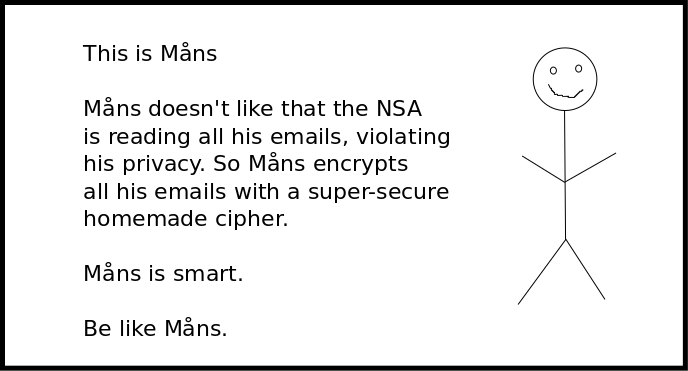
\includegraphics[width=\textwidth]{mans.png}
  \end{figure}
\end{center}

Måns har kommit på ett briljant chiffer för att skydda sig mot elakingar som försöker läsa hans epost. Hans chiffer fungerar på följande vis. Först använder han teckenkodningen ASCII för att representera varje tecken i sitt mail som ett tal mellan 0-127. Sedan väljer han en nyckel som består av $K$ bytes i intervallet 0-255. Om nyckeln består av bytes $a_0, a_1, a_2, ... a_{k - 1}$, och hans email består av bytes $b_0, b_1, b_2, ...$ så består krypteringen
av bytes $k_i = b_i \oplus a_{(i \mod K)}$, där $\oplus$ är en \href{https://en.wikipedia.org/wiki/Bitwise\_operation#XOR}{bitwise XOR} över de 8 bitarna i byten, och $i \mod K$ är den \href{https://en.wikipedia.org/wiki/Modulo\_operation}{sedvanliga modulo-operationen}. Slutligen kodar han varje byte som två tecken i bas 16 (\href{https://en.wikipedia.org/wiki/Hexadecimal}{hexadecimalt}).

Givet Måns krypterade meddelande, bestäm hur det ursprungliga meddelandet såg ut.

\section*{Indata}
Indata består av ett antal rader - det krypterade meddelandet. Observera att eventuella radbrytningar endast är med för att indata ska bli enklare att skriva, de ska inte tas hänsyn till i problemet.

Varje ursprungligt meddelande består av minst 500 och högst 1050 tecken.

\section*{Utdata}
Du ska skriva ut, tecken för tecken, Måns ursprungliga meddelande.

\section*{Poäng}

\begin{enumerate}
	\item[6 poäng] $K = 1$, meddelandet består enbart av små bokstäver $a-z$ och mellanslag.
	\item[10 poäng] $K = 1$.
  \item[12 poäng] $K \le 5$, texten består till 70\% av ordet \texttt{fisk}.
	\item[19 poäng] $K \le 5$, meddelandet består enbart av små bokstäver $a-z$ och mellanslag.
  \item[24 poäng] $K \le 5$
	\item[33 poäng] $K \le 10$, meddelandet består enbart av små bokstäver $a-z$ och mellanslag.
  \item[41 poäng] $K \le 10$
	\item[15 poäng] $K = 15$, ordet "flaggstangsknoppspoleringsmedel" förekommer i texten.
\end{enumerate}

I samtliga fall är det riktig text som krypterats, på antingen engelska, svenska eller tyska. Eventuella \href{https://sv.wikipedia.org/wiki/Diakritiskt\_tecken}{diakritiska tecken} har tagits bort.
